%----------------------------------------------------------------------------
We examine a three color optimal solution. For each run, a pulse sequence of the form shown in figure \ref{solution three pulses} is used where the amplitudes are selected in a uniform random fashion on the interval $[-20\%,+20\%]$ using the ``runif'' random number generator in MathCAD. Then a fourth-order Runge-Kutta fixed-step method is used to find the solution at 5001 points in the interval, and hence the residue ($\Psi_{residue}$) for each run. See figure \ref{three color optimum}.
%----------------------------------------------------------------------------
%----------------------------------------------------------------------------
% three_STIRAP.tex
% by Troy Hix, April 2005
%----------------------------------------------------------------------------
\begin{figure}
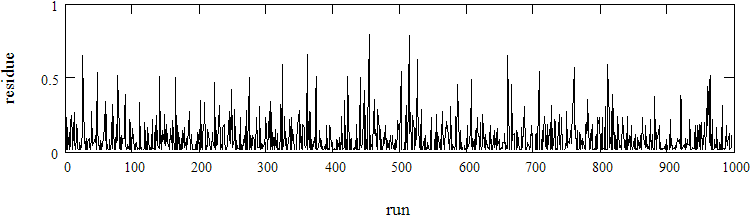
\includegraphics[width=6.00in]
{three_STIRAP/three_STIRAP.png}\\
\caption[Residue for runs using three color STIRAP]{Residue for runs using three color STIRAP. A pulse sequence of the form show in figure \ref{solution three pulses} is used here. The pulse amplitudes $A$, $B$, and $C$ varied uniformly on the interval $[-20\%,+20\%]$ for 1000 runs.}
\label{three color optimum}
\end{figure} 
%----------------------------------------------------------------------------

%----------------------------------------------------------------------------
%----------------------------------------------------------------------------
%----------------------------------------------------------------------------
%----------------------------------------------------------------------------
%----------------------------------------------------------------------------
%----------------------------------------------------------------------------
